

    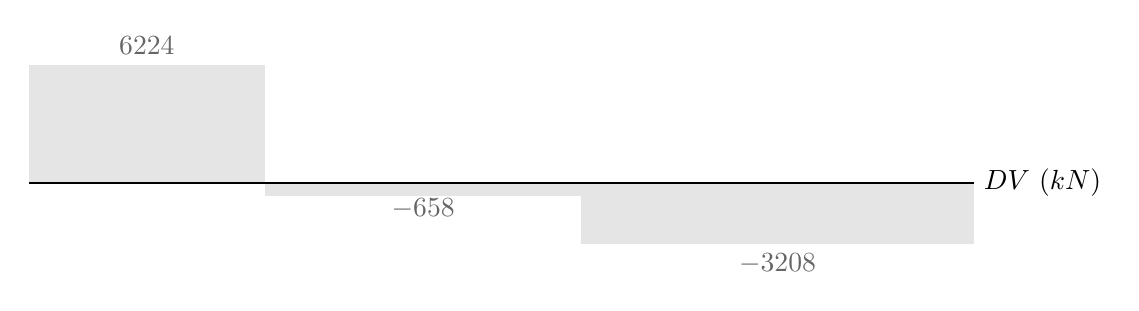
\begin{tikzpicture}
        % 1. VARIÁVEIS (Mantendo as mesmas proporções da viga anterior)
        \def\L{12}    % Comprimento total do diagrama (eixo x)
        \def\V{1.5}  % Altura do gráfico (representando a magnitude P/2)

        % 3. EIXO DE REFERÊNCIA (y = 0)
        % Linha que passa um pouco dos limites para indicar o eixo
        \draw[thick, gray] (0, 0) -- (\L, 0) node[right, text=black] {$DV \ (kN)$};

        % ==========================================
        % 4. ESFORÇO CORTANTE POSITIVO (0 até L/2)
        % ==========================================
        % Preenchimento com azul claro (20% de tinta azul, 80% branco)
        \fill[gray!20] (0,0) rectangle (\L/4, \V);

        % Rótulos da área positiva (Sinal de + e o valor P/2)
        \node[above, gray!80!black] at (\L/8, \V) {$6224$};

        % ==========================================
        % 5. ESFORÇO CORTANTE NEGATIVO (L/2 até L)
        % ==========================================
        % Preenchimento com vermelho claro
        \fill[gray!20] (\L/4,0) rectangle (\L/1.71, -0.11*\V);
        
        % Rótulos da área negativa (Sinal de - e o valor -P/2)
        \node[below, gray!80!black] at ({(\L/4 + \L/1.71)/2}, -0.11*\V/2) {$-658$};

        
        
        % Preenchimento com vermelho claro
        \fill[gray!20] (\L/1.71,0) rectangle (\L, -0.52*\V);
        
        % Rótulos da área negativa (Sinal de - e o valor -P/2)
        \node[below, gray!80!black] at ({(\L/1.71 + \L)/2}, -0.52*\V) {$-3208$};
        
        
        % Remarcando a linha base do diagrama em preto
        \draw[thick, black] (0,0) -- (\L,0);
    \end{tikzpicture}